\section{Обзор}

%На сегодняшний день, в области анализа динамически формируемого кода существует ряд различных подходов и инструментов, реализующих их~\cite{jsa, phpsa, alvor, varis, intelli}.
%В данной секции мы приводим краткий обзор методов, идеи которых переиспользуются нашим решением, а именно --- алгоритма синтаксического анализа регулярной аппроксимации и абстрактного синтаксического анализа. Помимо этого, нам потребовалось удобное представление контекстно-свободных грамматик в виде графа. Таким представлением стал Grammar Flow Graph~\cite{gfg}, описание которого также включено в обзор.

%На сегодняшний день, в области анализа динамически формируемого кода существует ряд различных подходов и инструментов, реализующих их~\cite{jsa, phpsa, alvor, varis, nastya, rnglr, a_lr}. Идея использования контекстно-свободной аппроксимации множества значений выражения была заимствована нами из статьи Y. Minamide, посвященной одному из таких инструментов --- PHPSA.  Для получения аппроксимации в PHPSA применяются стандартные методы анализа потока данных (dataflow analysis). Из исходного кода программы извлекается набор dataflow-уравнений, который интерпретируется как контекстно-свободная грамматика, описывающая язык, содержащий возможные значения выражения. Далее, решается вопрос о включении данного языка в эталонный, заданный пользователем при помощи другой КС-грамматики (с применением эвристик, т.к. в общем случае задача неразрешима).

Под \textit{контекстно-свободной аппроксимацией} подразумевается грамматика, описывающая контекстно-свободный язык, который содержит в качестве подмножества возможные значения динамически формируемого выражения. Идея использования такой аппроксимации была заимствована из существующих работ в области анализа динамически формируемого кода, краткий обзор которых будет приведен в данной секции. Алгоритм синтаксического анализа регулярной аппроксимации на основе GLL был адаптирован нами для работы c графовым представлением КС-грамматик. В качестве такого представления мы использовали Grammar Flow Graph (GFG,~\cite{gfg}). Описания оригинального алгоритма и GFG также включены в обзор. 

%Идея использования контекстно-свободной аппроксимации была заимствована из существующих работ в области анализа динамически формируемого кода, краткий обзор которых будет приведен в данной секции.
%Помимо этого, наше решение переиспользует модифицированный алгоритм обобщенного синтаксического анализа, позволяющий работать с нелинейным входом. 
%Его описание, а также описание графового представления контекстно-свободной аппроксимации, которое используется нашим алгоритмом, будут также представлены в отдельных параграфах.

%В данной секции приводится краткий обзор существующих подходов к анализу динамически формируемого кода. В отдельные параграфы выделены описание алгоритма синтаксического анализа регулярной аппроксимации, на котором основано наше решение, а также краткое изложение основных идей метода абстрактного синтаксического анализа, на которые мы будем ссылаться далее.

\subsection{Подходы к анализу динамически формируемых выражений}

Существует два основных подхода, позволяющих проводить различные виды анализа динамически формируемого кода. Один из них основан на проверке включения языка, аппроксимирующего множество значений динамически формируемого выражения, в эталонный контекстно-свободный язык, заданный пользователем. 
%в виде простого перечисления строк, либо при помощи грамматики. 
%Здесь под языком, который генерирует программа, подразумевается множество значений динамически формируемого выражения, а точнее, аппроксимирующее его множество.
%ведь в общем случае такое множество может быть рекурсивно перечислимым.
Данный подход был реализован в инструментах Java String Analyzer (JSA,~\cite{jsa}) и PHP String Analyzer (PHPSA,~\cite{phpsa}). %Для получения аппроксимации в них используются стандартные методы анализа потока данных (dataflow analysis). 
Получение аппроксимации в них реализовано следующим образом --- из исходного кода программы извлекается набор dataflow-уравнений, описывающих значения строковых переменных, которые участвуют в генерации выражения. Эти уравнения затем интерпретируются как контекстно-свободная грамматика, описывающая аппроксимирующий язык. PHPSA работает непосредственно с такой грамматикой, используя эвристики (т.к. в общем случае задача о включении КС-языков неразрешима~\cite{lang_inclusion}); в JSA контекстно-свободный язык дополнительно аппроксимируется регулярным.
%Из исходного кода программы извлекается набор dataflow-уравнений, который интерпретируется как контекстно-свободная грамматика, задающая аппроксимирующий язык. 


Другой подход заключается в проведении синтаксического анализа аппроксимации множества значений выражения. 
Такое решение позволяет не просто ответить на вопрос о включении языков, но и реализовать дополнительную функциональность, такую как вычисление семантики или рефакторинг. 
К методам, основанным на данном подходе, можно отнести алгоритмы синтаксического анализа регулярной аппроксимации на базе семейства GLR~\cite{alvor, rnglr_reg} и GLL-алгоритмов~\cite{gll_reg}, а также алгоритм абстрактного синтаксического анализа~\cite{a_lr}, позволяющий совместить синтаксический анализ с решением dataflow-уравнений, получаемых при помощи PHPSA.

\subsection{Синтаксический анализ регулярной аппроксимации на основе GLL}

Generalized LL (GLL)~\cite{gll} --- алгоритм синтаксического анализа, позволяющий, в отличие от классических LL-анализаторов, работать с произвольными контекстно-свободными грамматиками. 
При этом, GLL сохраняет такие важные свойства алгоритмов нисходящего разбора, как интуитивная связь с грамматикой и простота отладки и диагностики ошибок.

Основной идеей GLL является использование дескрипторов, позволяющих полностью описывать состояние анализатора в текущий момент времени.

\begin{definition}
    Дескриптор --- это четверка (L, u, i, N), где
    \begin{itemize}
        \setlength\itemsep{0em}
        \item L --- текущая позиция в грамматике вида $A \rightarrow \alpha \cdot \beta$
        \item u --- текущая вершина Graph Structured Stack (GSS,~\cite{tomita})
        \item i --- позиция во входном потоке
        \item N --- построенный на данный момент узел дерева вывода  
    \end{itemize}
\end{definition}  

В процессе работы поддерживается глобальная очередь дескрипторов. В начале каждого шага исполнения алгоритм берет следующий в очереди дескриптор и производит действия в зависимости от позиции в грамматике и текущего входного символа. 
Для обработки неоднозначностей в грамматике алгоритм добавляет дескрипторы для каждого возможного пути анализа в конец очереди. Результат работы алгоритма ---  множество деревьев разбора строки (лес разбора) --- представляется в виде Shared Packed Parse Forest (SPPF)~\cite{sppf}.

В рамках магистерской диссертации~\cite{gll_reg} на базе GLL был разработан алгоритм для синтаксического анализа регулярной аппроксимации множества значений динамически формируемого выражения. 
Под регулярной аппроксимацией здесь понимается детерминированный конечный автомат над алфавитом токенов (рис.~\ref{fig:app_r}). Оригинальный GLL-алгоритм был модифицирован для работы с нелинейным входом. 
Дескрипторы нового алгоритма хранят номер вершины входного графа вместо позиции в линейном потоке. Также, на шаге исполнения просматривается не единственный входной символ, а все ребра, исходящие из текущей вершины. Псевдокод данного алгоритма можно увидеть в приложении \ref{gll_code}. Основная логика работы представлена в функциях \textbf{dispatcher} (извлечение дескрипторов из очереди) и \textbf{processing} (анализ исходящих из текущей вершины ребер).

%\subsection{Абстрактный синтаксический анализ}

%В статьях~\cite{a_lr} Kyung-Goo Doh и David A. Schmidt представляют подход к работе с динамически формируемым кодом, который получил название \textit{абстрактный синтаксический анализ}. 
%Для аппроксимации множества значений формируемого выражения авторами было предложено использовать dataflow-уравнения, полученные из исходного кода программы (рис. \ref{dataflow_ex}). 
%Заметим, что эти уравнения представляют собой контекстно-свободную грамматику (рис. \ref{dataflow_ex}) --- нетерминальными символами будут имена переменных, терминалами --- строковые литералы. 
%Оператор объединения множеств означает, что для нетерминала существует несколько продукций. Грамматика, получаемая таким образом, в нашем подходе преобразуется в граф, который используется в качестве входного (по аналогии с графовым представлением конечного автомата из описанного ранее решения) для алгоритма синтаксического анализа.  

%В оригинальных статьях описан процесс решения системы уравнений методом поиска наименьшей неподвижной точки в домене LR-стеков, т.е. одновременно с решением производится синтаксический анализ с использованием стандартного LR(LALR)-автомата. 
%Результатом анализа является множество LR-стеков, представляющих различные варианты разбора выражения. Реализацию алгоритма в открытом доступе найти не удалось. Также, авторы не описывают возможность преобразования результатов в традиционное представление, такое как деревья синтаксического разбора, которое могло бы использоваться для более сложных видов анализа.

\subsection{Grammar Flow Graph}

%В качестве представления контекстно-свободной грамматики, которая является аппроксимацией множества значений выражения, мы используем Grammar Flow Graph (GFG)~\cite{gfg}. 
Grammar Flow Graph (GFG,~\cite{gfg}) --- связный помеченный граф, узлы которого соответствуют позициям в грамматике ($A \rightarrow \alpha \cdot \beta$). Различают следующие типы узлов ($X$ --- нетерминальный символ, $t$ --- терминальный):
\begin{itemize}
    \setlength\itemsep{-0.2em}
    \item[--] $A \rightarrow \alpha \cdot X \beta   $ --- call
    \item[--] $A \rightarrow \alpha X \cdot \beta$ --- return
    \item[--] $A \rightarrow \cdot \alpha$ --- entry
    \item[--] $A \rightarrow \alpha \cdot$ --- exit
    \item[--] $A \rightarrow \alpha \cdot t \beta$ --- scan
\end{itemize}
Для обозначения подграфа, представляющего продукции, имеющие в левой части нетерминал $A$, дополнительно используются узлы с метками $.A$ (start-узел) и $A.$ (end-узел). Подробное описание GFG можно найти в оригинальной статье.

Приведем определение выводимости строки в грамматике в терминах GFG. Для этого нам потребуется также определить понятие сбалансированного пути.

\begin{definition}
    Сбалансированным путем в GFG называется путь, подпоследователность call и return-узлов которого сбалансирована. 
\end{definition}

\begin{definition}
    Строка $w$ выводима в грамматике, если в GFG существует сбалансированный путь из узла $.S$ в узел $S.$ (здесь S --- стартовый нетерминал грамматики), и $w$ может быть получена конкатенацией меток на ребрах, содержащихся в данном пути. 
\end{definition}

\begin{figure}[h]
	\centering
	\begin{subfigure}[h!]{0.3\textwidth}
		\centering
		\begin{minipage}{4cm}
			\begin{Verbatim}[commandchars=\\\{\}]
x = \textcolor{red}{"a"}
while ...
    x = \textcolor{red}{"["} x \textcolor{red}{"]"}
print x
			\end{Verbatim}
		\end{minipage}
		\caption{Код}
		\label{fig:code}
	\end{subfigure}
	~
	\begin{subfigure}[h!]{0.3\textwidth}
		\centering
		$
		\begin{array}{crcl}
			&s' &::=& s \\
			&s & ::= & \mbox{\texttt{LBR }} s \mbox{\texttt{ RBR}}\\
			&s & ::= & \mbox{\texttt{A}}
		\end{array}
		$
		\caption{КС-аппроксимация}
		\label{fig:app_cf}
	\end{subfigure}
	~
	\begin{subfigure}[h!]{0.3\textwidth}
		\centering
		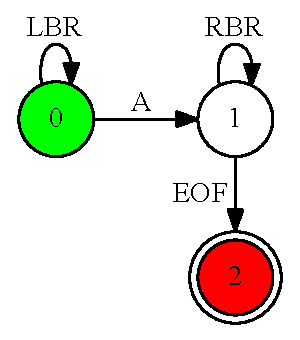
\includegraphics[width=2.5cm]{pictures/reg_app}
		\caption{Регулярная}
		\label{fig:app_r}
	\end{subfigure}
	\caption{Исходный код и примеры аппроксимаций}
	\label{example}
\end{figure}

\begin{figure}[h]
    \centering
    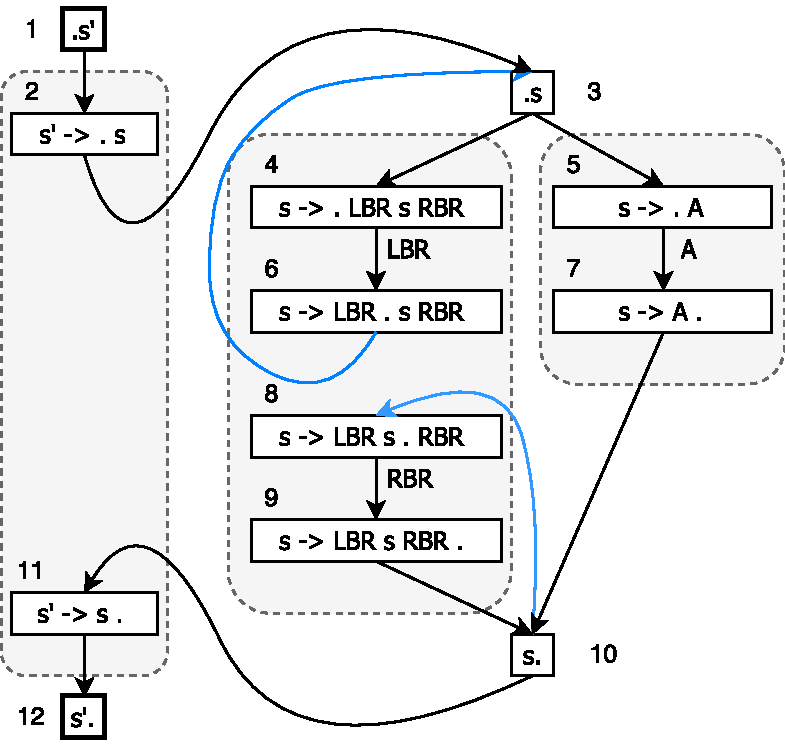
\includegraphics[width=0.5\textwidth]{pictures/gfg_enum}
    \caption{GFG для грамматики \ref{fig:app_cf}}
    \label{fig:gfg}
\end{figure}
